\documentclass[totpages,helvetica,openbib,italian]{europecv}
\usepackage[T1]{fontenc}
\usepackage{graphicx}
\usepackage[a4paper,top=1.27cm,left=1cm,right=1cm,bottom=2cm]{geometry}
\usepackage[italian]{babel}
\usepackage{bibentry}
\usepackage{url}

%\renewcommand{\ttdefault}{phv} % Uses Helvetica instead of fixed width font
\renewcommand{\normalsize}{\fontsize{8}{2}\selectfont}

\ecvname{Diego Russo}
\ecvaddress{Via G. Garibaldi 40, 05021, Acquasparta (TR), Italia}
\ecvtelephone[+39 334 5873886]{+39 0744 930614}
\ecvemail{\url{diegor.it@gmail.com} - Personale, gtalk, MSN \\& \url{diego.russo@forinicom.it} - Forinicom S.r.l.}
\ecvhomepage{\url{http://www.diegor.it}}
\ecvnationality{Italiana}
\ecvdateofbirth{30 aprile 1983}
\ecvgender{Maschio}
% \ecvbeforepicture{\raggedleft}
% \ecvpicture[width=3cm]{io}
% \ecvafterpicture{\ecvspace{-3.5cm}} 
\ecvfootnote{Per ulteriori informazioni: \url{http://europass.cedefop.eu.int}\\
\textcopyright~European Communities, 2003.}

\begin{document}
    \begin{center}
        \hspace{1pt}
        \vspace{2cm}
    
        {\scshape \textbf{\Huge Diego Russo}}
    
        \vspace{1cm}
    
        {\scshape \textbf{\large \underline{Curriculum Vitae}}}
    
        \vspace{0.25cm}
    
        aggiornato al \emph{\textbf{10 marzo 2010}}
        
        \vspace{2cm}
        
        \begin{figure}[htbp] 
            \begin{center} 
                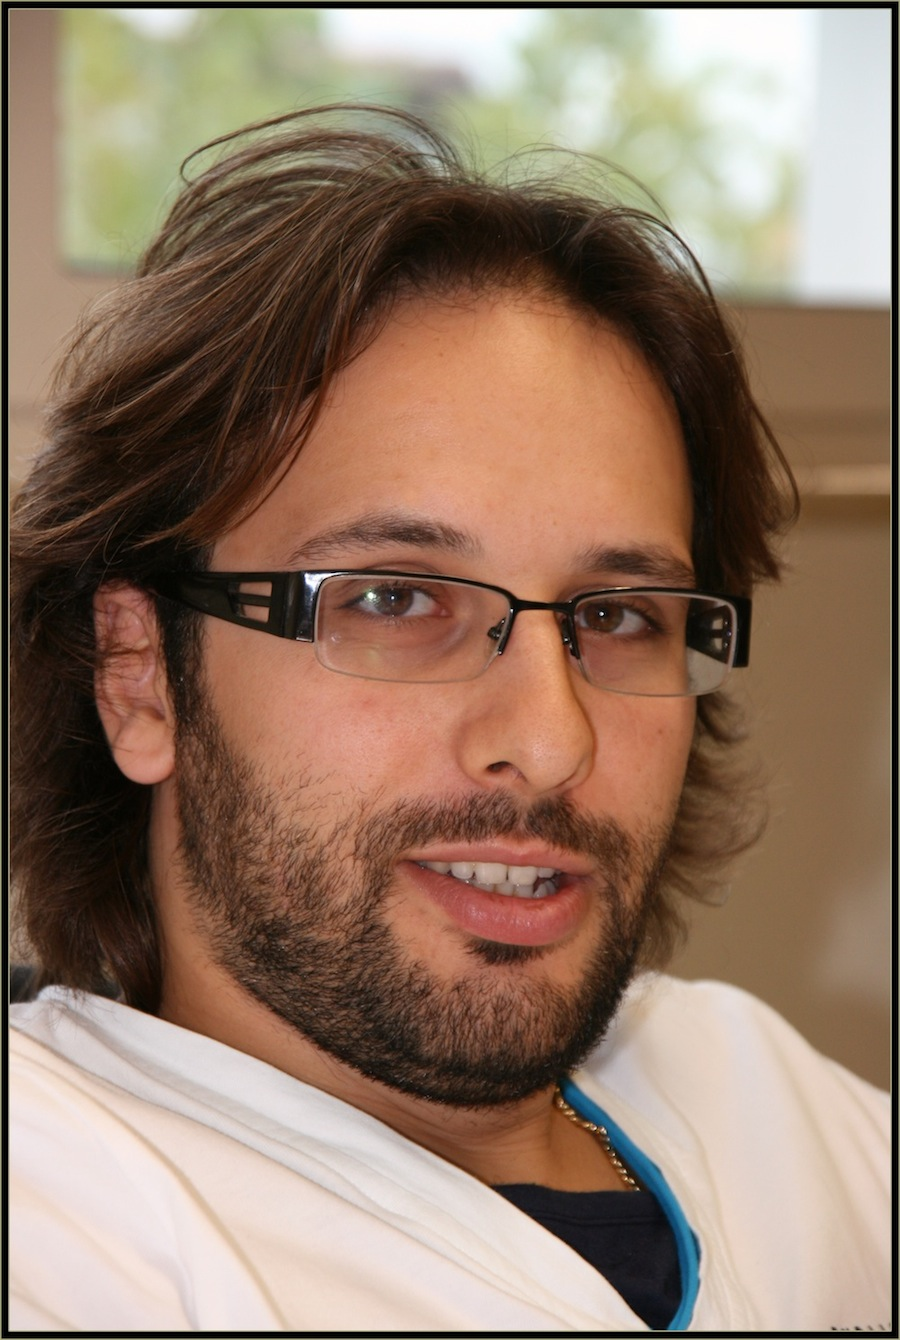
\includegraphics[width=10cm]{io.jpg}
            \end{center} 
        \end{figure}
        
    \end{center}
\pagebreak
\selectlanguage{italian}

\begin{europecv}
\ecvpersonalinfo[5pt]

%\ecvitem{\large\textbf{Impiego ricercato/ Settore di competenza}}{\large\textbf{Programmatore Python, Django.}}

\ecvsection{Esperienza professionale}

\ecvitem{Date}{\textbf{Dal 26 aprile 2008 ad Oggi}}
\ecvitem{Lavoro o posizione ricoperti}{Programmatore, sistemista (lavoratore con contratto di apprendistato part-time, 25 ore)}
\ecvitem{Principali attivit\'a e responsabilit\`a}{Sviluppo di un progetto che mira ad offrire connettivit\'a e servizi integrati (videosorveglianza, voip) alle pubbliche amministrazioni, aziende e privati. Punti previsti dal contratto:
\begin{itemize}
    \item conoscere i prodotti ed i servizi del settore e del contesto aziendale: reti Mesh e gararchiche, servizi VoIP e videosorveglianza, sicurezza delle reti wired e wireless;
    \item conoscere e saper applicare le basi tecniche e scientifiche della professionalit\'a;
    \item conoscere e saper utilizzare tecniche e metodi di lavoro con particolare riferimento allo sviluppo software e alla documentazione del codice;
    \item conoscere e saper utilizzare strumenti e tecnologie di lavoro (attrezzature, macchinari e strumenti di lavoro), in particolare ambiente di sviluppo Linux, piattaforma di sviluppo Eclipse, linguaggi di programmazione Python database MySQL e PostgresSQL;
    \item conoscere ed utilizzare misure di sicurezza individuale e per la tutela ambientale;
conoscere le innovazioni di prodotto, di processo, di contesto e di settore.
\end{itemize}}
\ecvitem{Nome e indirizzo del datore di lavoro}{Forinicom srl, Via del Popolo, 9 Bastia Umbra, 06083, 0758001868, \url{http://www.forinicom.it}}
\ecvitem{Tipo di attivit\`a o settore}{Settore telecomunicazioni}

\ecvitem[15pt]{}{}

\ecvitem{Date}{\textbf{Dal 03 settembre 2009 al 31 gennaio 2010}}
\ecvitem{Lavoro o posizione ricoperti}{Programmatore (lavoratore con contratto a progetto, part-time)}
\ecvitem{Principali attivit\'a e responsabilit\`a}{Sviluppo di un'applicazione gestionale per il comune di Bettona in django, python, postgresql, linux, apache, per l'informatizzazione dei servizi per la gestione delle anagrafiche nonch\'e delle pratiche edilizie ed urbanistiche e del calcolo della tassa ICI con aggiornamenti dei dati catastali. Utilizzo di un server per il controllo di versione (SVN), con relativa interfaccia web (trac) per la gestione dei ticket.}
\ecvitem{Nome e indirizzo del datore di lavoro}{Consorzio Miles - Servizi Integrati, CF 04881101002, Via Rocca di Papa 21, Roma}
\ecvitem{Tipo di attivit\`a o settore}{Servizi integrati per la pubblica amministrazione}
\ecvitem{}{}


\ecvsection{Istruzione e formazione}

\ecvitem{Date}{Iniziare con le informazioni pi\'u recenti ed elencare separatamente ciascun corso frequentato con successo. Facoltativo.}
\ecvitem{Certificato o diploma ottenuto}{\ldots}
\ecvitem{Principali materie/Competenze professionali apprese}{\ldots}
\ecvitem{Nome e tipo d'istituto di istruzione o formazione}{\ldots}
\ecvitem{Livello nella classificazione nazionale o internazionale\footnote{Se pertinente.}}{\ldots}

\ecvsection{Capacit\`a e competenze professionali}

\ecvmothertongue[80pt]{Precisare madrelingua/e}
\ecvitem{\large Altra/e lingua/e}{}
\ecvlanguageheader{(*)}
\ecvlanguage{Lingua}{\ecvAOne}{\ecvAOne}{\ecvATwo}{\ecvCOne}{\ecvCOne}
\ecvlastlanguage{Lingua}{\ecvCOne}{\ecvCOne}{}{}{\ecvCTwo}
\ecvlanguagefooter[10pt]{(*)}

\ecvitem[10pt]{Capacit\`a e competenze sociali}{Descrivere tali competenze e indicare dove sono state acquisite. Facoltativo.}
\ecvitem[10pt]{Capacit\`a e competenze organizzative}{Descrivere tali competenze e indicare dove sono state acquisite. Facoltativo.}
\ecvitem[10pt]{Capacit\`a e competenze tecniche}{Descrivere tali competenze e indicare dove sono state acquisite. Facoltativo.}
\ecvitem[10pt]{Capacit\`a e competenze informatiche}{Descrivere tali competenze e indicare dove sono state acquisite. Facoltativo.}
\ecvitem[10pt]{Capacit\`a e competenze artistiche}{Descrivere tali competenze e indicare dove sono state acquisite. Facoltativo.}
\ecvitem[10pt]{Altre capacit\`a e competenze}{Descrivere tali competenze e indicare dove sono state acquisite. Facoltativo.}
\ecvitem{Patente/i}{Indicare la(e) patente(i) di cui siete titolari precisandone la categoria. Facoltativo.}

\ecvsection{Ulteriori informazioni}
\ecvitem[10pt]{}{Inserire qui ogni altra informazione utile, ad esempio persone di riferimento, referenze, etc\ldots Facoltativo.}
\bibliographystyle{plain}
\nobibliography{publications}
% \ecvitem{}{\textbf{Pubblicazioni}}
% \ecvitem{}{\bibentry{pub1}}
% \ecvitem[10pt]{}{\bibentry{pub2}}
% \ecvitem{}{\textbf{Interessi personali}}
% \ecvitem{}{\ldots}  

\ecvsection{Allegati}
\ecvitem{}{Enumerare gli allegati al CV.}
\end{europecv}


\end{document} 